\documentclass[11pt,a4paper]{article}
\usepackage[margin=1in]{geometry}
\usepackage{graphicx}
\usepackage{amsmath,amssymb}
\usepackage{booktabs}
\usepackage{array}
\usepackage{url}
\usepackage{float}
\usepackage[numbers]{natbib}
\usepackage{tikz}
\usetikzlibrary{arrows.meta,positioning}
\usepackage[hidelinks]{hyperref}
\newcolumntype{L}[1]{>{\raggedright\arraybackslash}p{#1}}
\hypersetup{
  pdftitle={Real-Time MIDI Call-and-Response Generation Using Autoregressive Transformers},
  pdfauthor={Wang Zitong, Hu Sitong},
  pdfkeywords={symbolic music generation, MIDI, call-and-response, Transformer, temporal point process, real-time interaction, objective evaluation, blind listening, ablation study, latency logging, speculative preload}
}

\title{Real-Time MIDI Call-and-Response Generation Using Autoregressive Transformers}
\author{Wang Zitong, Hu Sitong}
\date{August 2026}

\begin{document}

\maketitle

\begin{abstract}
This paper tests whether an offline Anticipatory Music Transformer (AMT) can support real-time MIDI call-and-response without retraining. The primary contribution is an external adaptation architecture combining adaptive MIDI-VAD, phrase control, asynchronous playback, and speculative scheduling. A direct 100-call endpoint replay, a harmonized 27,000-row candidate comparison, a 63,000-row module ablation, an 18,000-row scheduler replay, and a blind study provide separate evidence. Under a fully specified structural-compliance composite, controlled AMT improves over shared-batch raw AMT from 0.560968 to 0.732610; style compliance accounts for much of the late-stage gain, while non-style structure rises from 0.558971 to 0.676704. Adaptive MIDI-VAD attains F1=0.712 at the stated two-second deadline, similar to fixed 800 ms (0.708) but with fewer premature commits (38 versus 68). A 150 ms pre-commit overlap reduces mean scheduler latency from 161.303 to 91.721 ms and underruns from 20.744\% to 5.244\%. Among 41 retained listeners, A4 is not rated conclusively above raw AMT, and the motif baseline is preferred to A6. The evidence supports an engineering adaptation and measurable structural control, not perceptual superiority or universally accurate turn segmentation.
\end{abstract}


\noindent\textbf{Keywords:} symbolic music generation; MIDI; call-and-response; Transformer; temporal point process; real-time interaction; objective evaluation; blind listening; ablation study; latency logging; speculative preload

\section{Introduction}
\label{sec:introduction}
Call-and-response is a foundational pattern in live improvisation, but realizing it computationally requires symbolic generators that can react on a performance clock rather than only complete offline continuations.

Autoregressive Transformers capture rich symbolic-music structure in offline generation, yet their stepwise decoding is poorly matched to live co-performance. Direct deployment creates four linked bottlenecks: synchronization with human timing, reliable phrase-end detection, latency spikes during inference, and structural degradation in high-entropy continuations. This paper therefore asks whether these limits can be reduced through external architecture and control layers without retraining the underlying model.

The \textbf{primary contribution} is the external system method: adaptive turn detection, phrase control, and speculative scheduling make a frozen offline AMT operable in a live MIDI loop. The stopping-time formulation is its turn-taking basis, while the endpoint benchmark, harmonized structural evaluation, module ablation, latency replay, and blind study are supporting tests with deliberately separate claim boundaries.


\section{Related Work}
\label{sec:related-work}

This section reviews the four areas that shape the proposed system: symbolic music representations, generative sequence models, real-time co-performance systems, and evaluation of generative music.

\subsection{Symbolic Music Representation}


Early symbolic music generation often used piano-rolls or fixed time-step grids, but rigid quantization can create sparse matrices and discard micro-timing such as rubato and swing \citep{boulanger2012modeling}. Event-based representations address this limitation through MIDI-like streams with \verb|Note-On|, \verb|Note-Off|, and relative \verb|Time-Shift| events \citep{oore2020feeling,huang2018musictransformer}. The Anticipatory Music Transformer further models symbolic music with temporal point-process events and asynchronous controls \citep{thickstun2023amt}. However, representation-level advances alone do not specify how continuous MIDI input should be segmented into interactive turns, especially when chords, hesitation pauses, and rubato-like timing occur in live performance.

\subsection{Sequence Models for Music Generation}

Symbolic music generation has moved from memoryless or recurrent models such as LSTMs \citep{eck2002finding} to self-attention-based Transformer architectures \citep{vaswani2017attention,huang2018musictransformer}. AMT extends this line toward controllable temporal-event generation \citep{thickstun2023amt}, but it remains primarily an offline model. Live co-performance adds endpoint detection, turn scheduling, and latency stability as deployment constraints. These models therefore do not directly address phrase-end detection or scheduler-level latency, which become necessary when offline symbolic generation is embedded into live interaction.

\subsection{Real-Time Human-AI Co-Performance}

Real-time human-AI co-performance systems must handle input capture, turn-taking, latency, and synchronization in addition to generation quality. MIDI-performance research emphasizes timing stability in interactive systems \citep{nelson2004midi}; Scramble Live illustrates the combination of learned models and live control in Max/MSP-style environments \citep{privato2022scramble}; and recent work couples Max/MSP front ends with Python generative back ends \citep{karchkhadze2026towards}. These systems show the importance of live control surfaces, but they leave open how an offline autoregressive symbolic model can be wrapped with endpoint logic, buffering, and fallback behavior without retraining. This study addresses that deployment gap through virtual MIDI routing and multithreaded asynchronous scheduling.

\subsection{Evaluation of Generative Music}

While human listening tests remain vital for evaluating musical quality, they are expensive and difficult to scale. Prior surveys emphasize that objective metrics for symbolic and generative music are useful for reproducible structural analysis, but they cannot fully replace perceptual or human-centered evaluation \citep{ji2023survey,lerch2025evaluation}. For real-time call-and-response, evaluation must also separate structural response quality from runtime behavior such as endpoint-to-first-MIDI latency and buffer underrun. The present evaluation therefore treats objective metrics, ablation evidence, scheduler logs, and a fixed-stimulus blind listening study as complementary rather than interchangeable forms of evidence.

\section{Temporal Point Process Modeling and Autoregressive Generation}
\label{sec:temporal-modeling}

\subsection{Continuous-Time MIDI Event Representation}

The performance is represented as a continuous-time event sequence
\begin{equation}
E=\{e_i=(t_i,d_i,p_i)\}_{i=1}^{N},\qquad
0\leq t_1\leq\cdots\leq t_N,
\end{equation}
where $t_i$ is onset time, $d_i>0$ is duration, and $p_i\in\{0,\ldots,127\}$ is MIDI pitch. Non-strict onset ordering permits chords; Section~\ref{sec:midi-vad-engineering} clusters near-simultaneous Note-On events before estimating onset density.

\subsection{Conditional Autoregressive Factorization}

For a human Call $C$ and response $R=\{e_j^r\}_{j=1}^{n}$, the frozen AMT decoder uses
\begin{equation}
P(R\mid C)=\prod_{j=1}^{n}P(e_j^r\mid C,e_{<j}^r),
\end{equation}
with event-level factorization
\begin{equation}
P(e_j^r\mid\cdot)=P(t_j^r\mid\cdot)
P(d_j^r\mid t_j^r,\cdot)
P(p_j^r\mid t_j^r,d_j^r,\cdot).
\end{equation}
The causal model supplies continuation probabilities; endpoint detection, scheduling, and phrase controls remain external and do not retrain its parameters.

\subsection{Dynamic Turn Segmentation Based on Continuous-Time Stopping Time}

Let $T_{\mathrm{last}}$ be the most recent Note-On and $\tau=t-T_{\mathrm{last}}$ the current silence. Under a point-process model with intensity $\lambda(t)$, the no-arrival probability is \citep{daley2003pointprocesses}
\begin{equation}
S(\tau)=\exp\left[-\int_0^{\tau}\lambda(T_{\mathrm{last}}+u)\,du\right].
\end{equation}
For the short online window, the implementation uses a local constant-rate approximation. If $u_1,\ldots,u_K$ are the most recent clustered onset times,
\begin{equation}
\mu_{\mathrm{tempo}}=
\max\left(0.25,\frac{K-1}{u_K-u_1}\right),
\qquad
S(\tau)=\exp(-\mu_{\mathrm{tempo}}\tau).
\end{equation}
With confidence boundary $\theta=0.05$, the candidate cutoff and stopping condition are
\begin{equation}
\tau_{\mathrm{cutoff}}=\frac{\ln(1/\theta)}{\mu_{\mathrm{tempo}}},
\label{eq:dynamic-cutoff}
\end{equation}
\begin{equation}
t-T_{\mathrm{last}}>\tau_{\mathrm{cutoff}}.
\label{eq:endpoint-condition}
\end{equation}
Thus the silence allowance shortens as recent onset density rises. This is an adaptive timer, not a proof of musical phrase completion; chord correction, revocable confirmation, and the direct endpoint benchmark in Section~\ref{subsec:endpoint-benchmark} define and test its operational behavior.


\section{Real-Time MIDI Call-and-Response System Design}
\label{sec:system-design}

\subsection{Cross-Environment Architecture Based on Virtual MIDI }

The system uses a modular Virtual MIDI Bus architecture rather than a monolithic offline-generation pipeline. Physical MIDI input, host audio rendering, neural inference, and MIDI output scheduling are decoupled so that equivalent routing chains can be used across operating systems and digital audio workstations.

In Windows, the routing chain can use loopMIDI with REAPER, Decent Sampler, or another host; in macOS, it can use the IAC Bus with Logic Pro or an equivalent DAW. The system is therefore defined by the interaction chain itself: physical MIDI input, virtual MIDI routing, a Python inference engine, and host-based rendering.

Figure~\ref{fig:System_overview} separates MIDI capture and host rendering from the Python back end, which maintains the Call buffer, detects endpoints, decodes asynchronously, applies phrase controls, schedules playback, and writes diagnostic logs.

\begin{figure}[H]
\centering
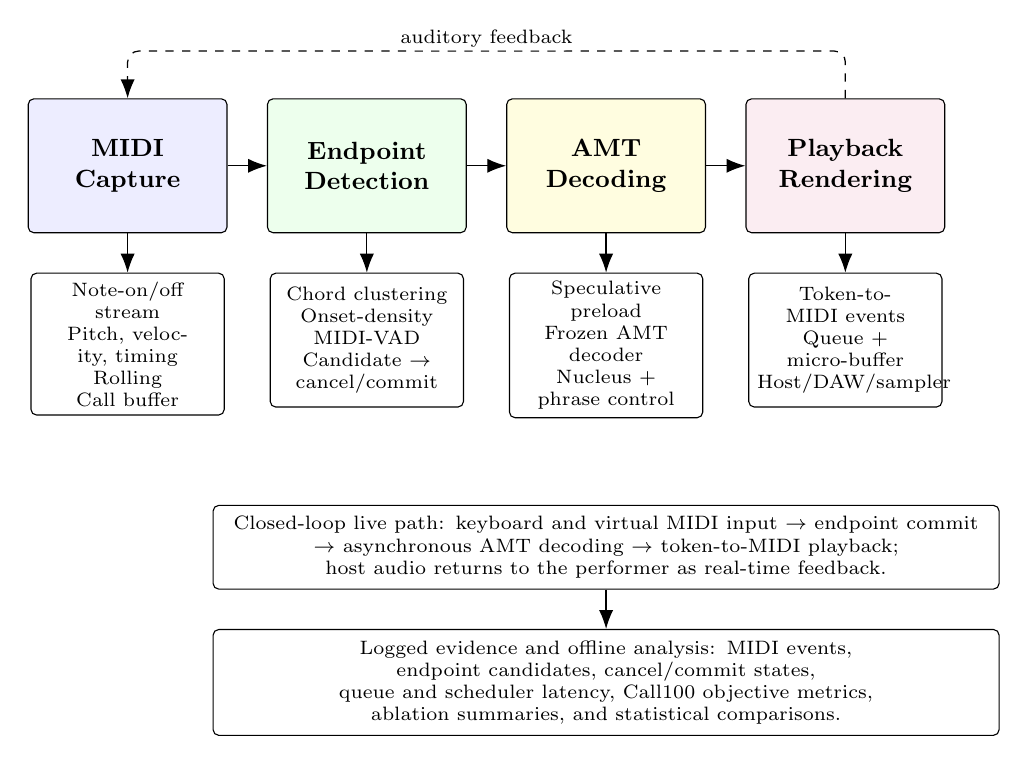
\begin{tikzpicture}[
    node distance=5mm,
    stage/.style={draw, rounded corners=2pt, align=center, text width=0.185\linewidth, minimum height=17mm, inner sep=4pt, font=\small\bfseries},
    detail/.style={draw, rounded corners=2pt, align=center, text width=0.185\linewidth, minimum height=17mm, inner sep=3pt, font=\scriptsize},
    side/.style={draw, rounded corners=2pt, align=center, text width=0.80\linewidth, minimum height=10mm, inner sep=4pt, font=\scriptsize},
    arrow/.style={-{Latex[length=2.4mm]}, line width=0.45pt},
    feedback/.style={-{Latex[length=2.4mm]}, line width=0.45pt, dashed, rounded corners=4pt}
]
\node[stage, fill=blue!7] (capture) {MIDI Capture};
\node[stage, fill=green!7, right=of capture] (endpoint) {Endpoint Detection};
\node[stage, fill=yellow!12, right=of endpoint] (generation) {AMT\\Decoding};
\node[stage, fill=purple!7, right=of generation] (playback) {Playback Rendering};

\node[detail, below=of capture] (captureD) {Note-on/off stream\\Pitch, velocity, timing\\Rolling Call buffer};
\node[detail, below=of endpoint] (endpointD) {Chord clustering\\Onset-density MIDI-VAD\\Candidate $\rightarrow$ cancel/commit};
\node[detail, below=of generation] (generationD) {Speculative preload\\Frozen AMT decoder\\Nucleus + phrase control};
\node[detail, below=of playback] (playbackD) {Token-to-MIDI events\\Queue + micro-buffer\\Host/DAW/sampler};

\draw[arrow] (capture) -- (endpoint);
\draw[arrow] (endpoint) -- (generation);
\draw[arrow] (generation) -- (playback);
\draw[feedback] (playback.north) -- ++(0,6mm) -- node[midway, above, fill=white, inner sep=1pt, font=\scriptsize] {auditory feedback} ([yshift=6mm]capture.north) -- (capture.north);
\draw[arrow] (capture) -- (captureD);
\draw[arrow] (endpoint) -- (endpointD);
\draw[arrow] (generation) -- (generationD);
\draw[arrow] (playback) -- (playbackD);

\node[side, below=11mm of generationD] (loop) {Closed-loop live path: keyboard and virtual MIDI input $\rightarrow$ endpoint commit\\$\rightarrow$ asynchronous AMT decoding $\rightarrow$ token-to-MIDI playback;\\host audio returns to the performer as real-time feedback.};
\node[side, below=of loop] (eval) {Logged evidence and offline analysis: MIDI events, endpoint candidates, cancel/commit states,\\queue and scheduler latency, Call100 objective metrics,\\ablation summaries, and statistical comparisons.};

\draw[arrow] (loop.south) -- (eval.north);
\end{tikzpicture}
\caption{System overview of the real-time MIDI call-and-response framework. The figure shows the four online stages, the auditory feedback loop, and the logged evidence used for offline evaluation.}
\label{fig:System_overview}
\end{figure}

The online path is therefore capture $\rightarrow$ candidate/commit $\rightarrow$ AMT decoding $\rightarrow$ MIDI playback. Speculative work may begin at a candidate, but only committed Calls enter the audible path; canceled work is discarded.

\subsection{Engineering Implementation of the Intelligent MIDI Endpoint Detection Module}
\label{sec:midi-vad-engineering}

The MIDI-VAD daemon polls Note-On events, updates the clustered onset window, and evaluates Equations~\eqref{eq:dynamic-cutoff}--\eqref{eq:endpoint-condition}. Its state machine is
\begin{equation}
\text{Listening}
\rightarrow
\text{Candidate}
\rightarrow
\begin{cases}
\text{Cancel} \rightarrow \text{Listening},\\
\text{Commit} \rightarrow \text{Inference}.
\end{cases}
\label{eq:midi-vad-state-machine}
\end{equation}
where a new Note-On cancels an unconfirmed candidate; commit freezes the Call for inference.

\subsubsection{Chord-Clustering Correction for Onset-Density Estimation}

Counting every note in a chord would inflate $\mu_{\mathrm{tempo}}$. Note-On events within
\begin{equation}
\Delta t_{\mathrm{cluster}} \approx 0.08\,\mathrm{s}.
\label{eq:cluster-window}
\end{equation}
are merged into one onset cluster. The value is an engineering setting, not a learned constant. Online accompaniment work explicitly allows imperfect performance detection \citep{dannenberg1984online}; related MIDI voice separation groups onsets within 35 ms and separately uses an 80 ms busy-note allowance after onset-group time \citep{madsen2006separating}. Neither value transfers directly to this detector. Here 80 ms corrects density only, and Section~\ref{subsec:endpoint-benchmark} tests 0, 40, 80, and 120 ms sensitivity rather than treating it as universal.

\subsubsection{Two-Stage Revocable Candidate Endpoint and Confirmation Window}
\label{sec:revocable-endpoint}

When Equation~\eqref{eq:endpoint-condition} is first satisfied, the system records $T_{\mathrm{candidate}}$ and waits
\begin{equation}
\Delta T_{\mathrm{confirm}} \approx 0.15\,\mathrm{s}.
\label{eq:confirm-window}
\end{equation}
A Note-On within this interval cancels the candidate; otherwise it commits. The 150 ms value is not a perceptual threshold. Synchronous music can demand roughly 20--30 ms latency \citep{lago2004quest}, while tolerance varies strongly with task and feedback topology \citep{rottondi2016overview}. For this turn-taking system, 150 ms is a debounce/latency compromise tested against 0, 75, and 250 ms in Section~\ref{subsec:endpoint-benchmark}; preload can overlap, but not extend beyond, this same interval.
\subsection{Asynchronous Streaming Decoding and Micro-Buffered Scheduling}
\label{sec:streaming-decoding}

An inference thread places playable events in a thread-safe queue while a playback thread converts them to MIDI. Playback begins after an 80 ms micro-buffer. For generated event duration $D(y_k)$ and per-event inference time $\tau_{\mathrm{infer}}(k)$, an underrun is avoided while
\begin{equation}
\Delta T_{\mathrm{buffer}}
+
\sum_{k=1}^{j} D(y_k)
>
\sum_{k=1}^{j+1} \tau_{\mathrm{infer}}(k),
\quad
\forall j \in \{1,2,\ldots,n-1\}.
\label{eq:streaming-buffer-condition}
\end{equation}
This overlap changes scheduling, not intrinsic AMT inference time.

\subsubsection{Speculative Preload for Candidate Endpoints}
\label{sec:speculative-preload}

At candidate time, the engine snapshots the Call and may start decoding while MIDI monitoring continues. A commit reuses available tokens; a cancel discards them. The scheduler model used in Section~\ref{subsec:latency-logging} is
\begin{equation}
L_{\mathrm{first}}
=
\max\left(
0,\,
\tau_{\mathrm{first}}-\Delta T_{\mathrm{confirm}}
\right)
+\Delta T_{\mathrm{buffer}}.
\label{eq:perceived-latency-preload}
\end{equation}
Here $\tau_{\mathrm{first}}$ is time to the first playable token. Because $\Delta T_{\mathrm{preload}}=\Delta T_{\mathrm{confirm}}=150$ ms, no 250 ms post-confirmation horizon exists: preload occupies only the revocable candidate interval. Canceled candidates trade temporary computation for lower committed-path delay.

\subsection{Relative Interval Representation and Nucleus Sampling Control in a High-Entropy Setting}
\label{sec:relative-interval-nucleus-sampling}

The decoder receives relative timing and pitch movement,
\begin{equation}
\Delta t_i=t_i-t_{i-1},\qquad \Delta p_i=p_i-p_{i-1},
\label{eq:relative-arrival-time}
\end{equation}
and applies temperature-scaled nucleus sampling \citep{holtzman2020curious}. For sorted token probabilities $P_T(x_{(i)})$, it retains the smallest prefix satisfying
\begin{equation}
K =
\min \left\{
k
\ \middle|\
\sum_{i=1}^{k} P_T(x_{(i)}) \geq p
\right\}.
\label{eq:nucleus-k}
\end{equation}
where $p$ is preset-dependent (typically 0.95) and
\begin{equation}
P_T(x_i)
=
\frac{\exp(z_i/T)}
{\sum_j \exp(z_j/T)}.
\label{eq:temperature-scaling}
\end{equation}
These controls reshape sampling but impose no tonal rule; tonal and metrical projection, when enabled, occurs later in the explicit style layer.
\subsection{Phrase-level Music Control Layer}
\label{sec:phrase-level-control}

The phrase controller derives global limits from the Call, rejects repetition failures during sampling, matches response duration, and supplies a deterministic fallback only when no playable neural output exists. It remains external to AMT parameters.

\subsubsection{CallProfile-based Phrase Intention Analysis and ResponsePlan Construction}
\label{sec:callprofile-responseplan}

After commit, the CallProfile is
\begin{equation}
P_{\mathrm{call}}
=
\left[
T_{\mathrm{call}},
N_{\mathrm{call}},
\Omega_{\mathrm{pitch}},
\bar{p}_{\mathrm{call}},
H_{\mathrm{pitch}},
\nabla_{\mathrm{melody}},
\rho_{\mathrm{rhythm}},
T_{\mathrm{repeat}}
\right]^T.
\label{eq:callprofile-vector}
\end{equation}
The terms encode duration, note count, pitch range and mean, pitch-class distribution, first-order contour, onset density, and repeated-tail status. They produce
\begin{equation}
\mathrm{Plan}_{\mathrm{resp}}
=
\left\{
T_{\mathrm{target}},
N_{\mathrm{target}},
\Omega_{\mathrm{allow}},
CPR_{\mathrm{limit}},
Share_{\max},
K_{\mathrm{resample}}
\right\}.
\label{eq:responseplan}
\end{equation}
which fixes target duration/note count, allowed register, continuous-repetition and dominant-pitch limits, and the resampling budget.

\subsubsection{Repetition-tail Compression and Repetition Suppression}
\label{sec:repetition-tail-suppression}

A repeated Call tail (at least three same-pitch events or dominance in the final window) is compressed to at most two prompt events. During decoding, a token is rejected if it would exceed either $CPR_{\mathrm{limit}}$ consecutive equal pitches or dominant-pitch share $Share_{\max}$. Rejection is retried up to $K_{\mathrm{resample}}$ times; exhaustion invokes a nearby consonant event-level repair around $\bar p_{\mathrm{call}}$. This repair is distinct from the whole-phrase motif fallback below.

\subsubsection{Motif-transformation Fallback and Duration Matching}
\label{sec:fallback-duration-matching}

\noindent\textbf{(1) Whole-phrase fallback trigger and mapping.}
The motif generator is called only when decoding returns zero playable events and fallback is enabled. Rejected individual events instead use the event-level repair described above; they do not replace the phrase. For an empty response, the live system transforms the cleaned Call tail:
\begin{equation}
R_{\mathrm{fallback}}
=
T_{\mathrm{scale}}
\circ T_{\mathrm{clip}}
\circ T_{\mathrm{shift}}
\circ T_{\mathrm{inverse}}
(C_{\mathrm{tail}}).
\label{eq:motif-fallback}
\end{equation}

Here $C_{\mathrm{tail}}$ is the last $\min(N_{\mathrm{call}},N_{\mathrm{target}})$ notes after prompt cleaning. The live fallback preserves their chronological order and maps each $e_i=(t_i,d_i,p_i)$ to
\begin{equation}
\hat{t}_i
=
T_{\mathrm{end}}(C)
+
\lambda
\left(
t_i - t_{\mathrm{tail},0}
\right),
\qquad
\hat{d}_i
=
\mathrm{clip}
\left(
\lambda d_i,\,
d_{\min},\,
d_{\max}
\right),
\label{eq:fallback-time-rule}
\end{equation}
where $T_{\mathrm{end}}(C)$ is the end time of the Call, $t_{\mathrm{tail},0}$ is the first onset in the selected tail, and
\begin{equation}
\lambda =
\max\left(0.2,\frac{T_{\mathrm{target}}}
{\max(T_{\mathrm{tail}}, \epsilon)}\right).
\label{eq:fallback-scale}
\end{equation}
Pitch is generated by inversion around the Call mean pitch and a small contour shift:
\begin{equation}
\hat{p}_i
=
\mathrm{clip}
\left(
2\bar{p}_{\mathrm{call}} - p_i + \delta,\,
p_{\min}^{\mathrm{allow}},\,
p_{\max}^{\mathrm{allow}}
\right).
\label{eq:fallback-pitch-rule}
\end{equation}
For live fallback, $\delta=-5$ semitones for descending Calls and $+5$ otherwise. Durations are clipped to configured minima/maxima; rejected fallback events pass through the same repetition repair before acceptance. The offline motif baseline, also used by the A4 branch if it is ever activated, selects the tail under the fixed experiment seed, uses $\delta\in\{-5,-3,2,3,5,7\}$, applies the same pitch-share safeguards, re-sorts by onset, and finally applies the chosen style projection. Section~\ref{subsec:controlled-amt-ablation} reports activation separately from event repairs.

\noindent\textbf{(2) Response duration matching.}
Before rendering, duration matching computes
\begin{equation}
T_{\mathrm{raw}} = \max_i(t_i^r+d_i^r)-\min_i t_i^r.
\label{eq:raw-response-duration}
\end{equation}
\begin{equation}
\gamma =
\frac{T_{\mathrm{target}}}{T_{\mathrm{raw}}}.
\label{eq:duration-match-ratio}
\end{equation}
If $T_{\mathrm{raw}}\in[0.80T_{\mathrm{target}},1.25T_{\mathrm{target}}]$, only duration bounds are enforced. Longer responses use bounded proportional scaling. Shorter responses mix normalized original onset position $q_i$ with sequence position $i/(n-1)$:
\begin{equation}
q_i'=(1-\beta)q_i+\beta\frac{i}{n-1},
\qquad
\beta=\operatorname{clip}\left(0.35+0.45\left(1-\frac{S_{\mathrm{raw}}}{S_{\mathrm{target}}}\right),0.35,0.80\right),
\label{eq:actual-onset-time}
\end{equation}
\begin{equation}
d_i'=\operatorname{clip}\left(d_i\min\left(2,\frac{T_{\mathrm{target}}}{T_{\mathrm{raw}}}\right),d_{\min},d_{\max}\right).
\label{eq:actual-duration}
\end{equation}
Here $S$ denotes onset span. Raw duration, adjusted duration, and stretch factor are logged for ablation analysis.

\subsection{Chromatic Free Improvisation and Optional Style Constraint Layer}

Chromatic mode leaves pitch class and rhythmic grid unconstrained. The optional \texttt{pentatonic\_\allowbreak 2bar\_\allowbreak 4\_\allowbreak 4} post-processor instead makes a specific style contract explicit; it does not change AMT probabilities.

\subsubsection{Chromatic Mode}

This default retains nucleus sampling and phrase safety controls but applies no hard scale, cadence, meter, or quantization rule.

\subsubsection{Engineering Implementation of the pentatonic\_2bar\_4\_4 Style Constraint Layer}

The constrained mode applies five deterministic stages: (i) truncate to eight beats in 4/4; (ii) project pitch to
\begin{equation}
P_{\mathrm{pent}}=\{p\in\mathbb Z:(p\bmod 12)\in M_{\mathrm{mode}}\},
\qquad p_i'=\Pi_{P_{\mathrm{pent}}}(p_i);
\end{equation}
(iii) quantize onset and duration to the selected grid,
\begin{equation}
t_i'=\Delta t_{\mathrm{grid}}\operatorname{round}(t_i/\Delta t_{\mathrm{grid}});
\end{equation}
(iv) move unstable notes on beats one and three toward stable degrees; and (v) correct the final cadence and fold or replace any interval exceeding $\Delta p_{\max}$. These same targeted rules motivate separating style compliance from non-style structure in the evaluator.

\section{Experimental Design, Objective Evaluation, and Blind Listening}
\label{sec:call100-evaluation}

The evaluation follows five claim-specific layers: endpoint segmentation, candidate comparison, module attribution, scheduler replay, and fixed-stimulus listening. No layer is treated as a substitute for another.

\subsection{Experiment Hierarchy and Evaluation Goals}
\label{subsec:eval-goals}

The evaluation is organized to avoid a single-score interpretation of the system. Because the proposed method combines musical control, module-level engineering, and runtime scheduling, each claim is tested at the level where it can be observed most directly. Figure~\ref{fig:evidence-chain} summarizes this structure before the individual datasets, metrics, and results are introduced.

\begin{figure}[H]
\centering
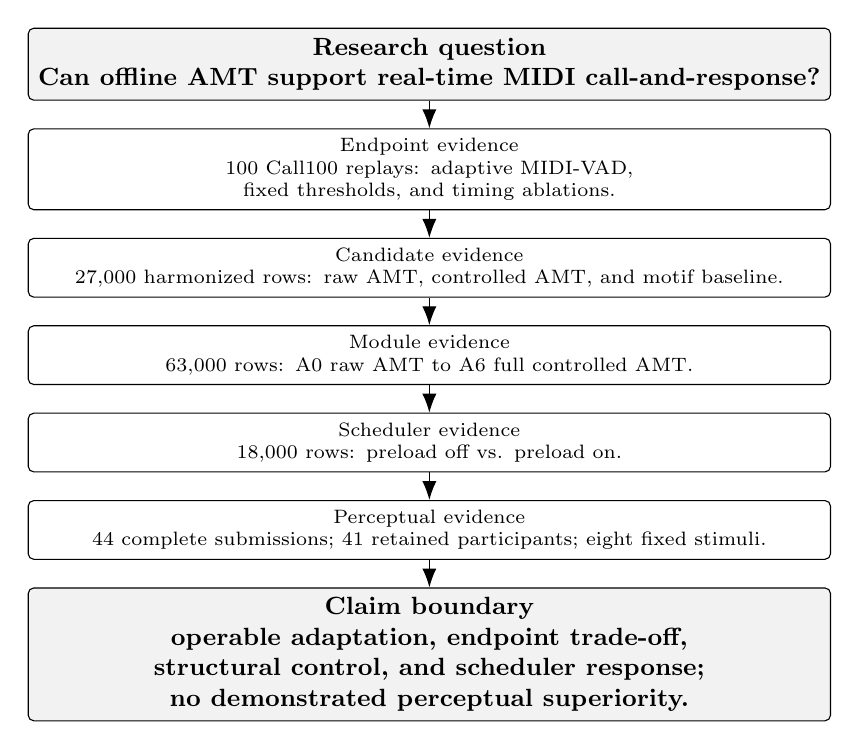
\begin{tikzpicture}[
    node distance=3.5mm,
    evidence/.style={draw, rounded corners=2pt, align=center, text width=0.82\linewidth, inner sep=3.5pt, font=\scriptsize},
    claim/.style={draw, rounded corners=2pt, align=center, text width=0.82\linewidth, inner sep=3.5pt, font=\small\bfseries, fill=gray!10},
    arrow/.style={-{Latex[length=2.4mm]}, line width=0.45pt}
]
\node[claim] (main) {Research question\\Can offline AMT support real-time MIDI call-and-response?};
\node[evidence, below=of main] (layer0) {Endpoint evidence\\100 Call100 replays: adaptive MIDI-VAD, fixed thresholds, and timing ablations.};
\node[evidence, below=of layer0] (layer1) {Candidate evidence\\27,000 harmonized rows: raw AMT, controlled AMT, and motif baseline.};
\node[evidence, below=of layer1] (layer2) {Module evidence\\63,000 rows: A0 raw AMT to A6 full controlled AMT.};
\node[evidence, below=of layer2] (layer3) {Scheduler evidence\\18,000 rows: preload off vs. preload on.};
\node[evidence, below=of layer3] (layer4) {Perceptual evidence\\44 complete submissions; 41 retained participants; eight fixed stimuli.};
\node[claim, below=of layer4] (supported) {Claim boundary\\operable adaptation, endpoint trade-off, structural control, and scheduler response;\\no demonstrated perceptual superiority.};
\draw[arrow] (main) -- (layer0);
\draw[arrow] (layer0) -- (layer1);
\draw[arrow] (layer1) -- (layer2);
\draw[arrow] (layer2) -- (layer3);
\draw[arrow] (layer3) -- (layer4);
\draw[arrow] (layer4) -- (supported);
\end{tikzpicture}
\caption{Experiment hierarchy and evidence chain.}
\label{fig:evidence-chain}
\end{figure}

Endpoint replay tests turn segmentation directly; the remaining layers test structural control, module attribution, scheduler behavior, and listener preference in that order. The primary system claim therefore does not depend on interpreting the structural composite as perceived musical quality.

\subsection{Construction of the Call100 Benchmark}
\label{subsec:call100-dataset}

Call100 contains 100 call phrases and extends early demonstrations into a mixed-distribution robustness test. It is built in two stages. First, it reuses Call50 without modifying its files: 10 artificial stress-test calls and 40 real public MIDI fragments. The artificial calls deliberately probe likely failure modes, including clear motifs, minor-pentatonic questions, blues or chromatic tension, half cadences, repeated tails, syncopation, sparse long tones, dense eighth-note motion, arch contours, and large leaps followed by stepwise filling.

The 40 real calls in Call50 are extracted from POP909 \citep{wang2020pop909} using a conservative two-bar melody-sampling procedure. The extraction script scans MIDI tracks with melody-like names such as \texttt{melody}, \texttt{main}, \texttt{vocal}, and \texttt{lead}, while excluding tracks that are more likely to represent accompaniment or percussion, such as \texttt{chord}, \texttt{bass}, and \texttt{drum}. Candidate windows are two bars long, corresponding to 8 beats, and the window advances by 2 beats. A candidate is kept only if it contains between 6 and 24 notes, has a polyphonic-overlap ratio no greater than 0.10, and reaches a major/minor scale-fit score of at least 0.85. A fixed random seed, 20260529, is then used to shuffle the candidates and select 40 real snippets reproducibly.

Second, Call100 copies Call50 into a new benchmark directory and adds 50 public MIDI excerpts without rewriting the original \texttt{calls\_50} directory. In the reproducible run reported here, the available public source was POP909, so all additions come from POP909. The builder constructs two-bar windows from tracks such as \texttt{MELODY}, \texttt{BRIDGE}, and \texttt{PIANO}, computes descriptive features, scores candidates against eight diagnostic target categories, and applies fingerprint deduplication.

Table~\ref{tab:call100-dataset} summarizes the source distribution, Call50 origins, and public-addition targets. The benchmark is diagnostic rather than corpus-representative: it preserves artificial stress cases while adding public excerpts for broader melodic input. Planned MAESTRO, ASAP, Lakh/Slakh, and GiantMIDI sources were not locally available, so the dataset report records their absence and the public additions are backfilled from POP909.

\begin{table}[htbp]
\centering
\caption{Detailed composition of the Call100 benchmark}
\label{tab:call100-dataset}
\small
\begin{tabular}{>{\raggedright\arraybackslash}p{0.20\linewidth}>{\raggedright\arraybackslash}p{0.26\linewidth}r>{\raggedright\arraybackslash}p{0.37\linewidth}}
\toprule
Source or origin & Subset or target type & Calls & Purpose or selection rule \\
\midrule
\texttt{calls\_50} & Artificial stress tests & 10 & Hand-designed edge cases: pentatonic motif, minor question, blues/chromatic tension, half cadence, repetition tail, syncopation, sparse long tones, dense motion, arch contour, and leap gap filling. \\
\texttt{calls\_50} & Real POP909 snippets & 40 & Two-bar monophonic melody windows from melody-like tracks; 6--24 notes, overlap ratio $\leq 0.10$, scale fit $\geq 0.85$, seed 20260529. \\
\midrule
\texttt{POP909} & Clear motif & 12 & Public additions selected for stable motivic structure. \\
\texttt{POP909} & Expressive rubato & 8 & Irregular timing and flexible inter-onset intervals. \\
\texttt{POP909} & Chord/arpeggio texture & 8 & Chordal or partially polyphonic input gestures. \\
\texttt{POP909} & Sparse short phrase & 5 & Low-information calls with few notes or long gaps. \\
\texttt{POP909} & Dense fast motion & 5 & High onset density and faster melodic movement. \\
\texttt{POP909} & Chromatic outside notes & 5 & Lower scale-fit or chromatic-tension cases. \\
\texttt{POP909} & False-ending pause & 4 & Internal or trailing pauses that may confuse endpoint detection. \\
\texttt{POP909} & Repetition tail & 3 & Repeated endings that may trigger response repetition. \\
\midrule
Total & Call100 benchmark & 100 & 10 artificial stress calls, 40 real Call50 snippets, and 50 public POP909 additions. \\
\bottomrule
\end{tabular}
\end{table}

\subsection{Candidate Strategies and Parameter Presets}
\label{subsec:candidates-presets}

The formal experiment compares three candidate strategies, summarized in Table~\ref{tab:candidate-strategies}. The raw AMT condition directly uses the pretrained AMT decoder without external phrase-level control. The controlled AMT condition keeps the same decoder but adds call profiling, prompt cleaning, repetition suppression, fallback generation, and duration matching. The motif baseline does not use a neural decoder; instead, it produces responses through rule-based motif transformation and is treated as a strong structural baseline.

\begin{table}[htbp]
\centering
\caption{Candidate strategies in the Call100 experiment}
\label{tab:candidate-strategies}
\small
\begin{tabular}{L{0.34\linewidth}L{0.52\linewidth}}
\toprule
Candidate ID & Description \\
\midrule
\texttt{amt\_small\_raw} & Raw AMT response generation without external phrase-level control. \\
\texttt{amt\_small\_controlled} & AMT response generation with call profiling, repetition suppression, fallback generation, and duration matching. \\
\texttt{motif\_transform\_baseline} & Rule-based motif transformation baseline used as a strong non-neural comparison. \\
\bottomrule
\end{tabular}
\end{table}

The experiment uses six parameter presets, listed in Table~\ref{tab:parameter-presets}. Each call, preset, and candidate combination is run for 15 trials. The total experiment scale is therefore:

\begin{equation}
100 \;\mathrm{calls} \times 6 \;\mathrm{presets} \times 3 \;\mathrm{candidates} \times 15 \;\mathrm{trials}
= 27000.
\end{equation}

\begin{table}[htbp]
\centering
\caption{Parameter presets used in the Call100 experiment}
\label{tab:parameter-presets}
\small
\begin{tabular}{ll}
\toprule
Preset group & Preset ID \\
\midrule
No-theory control & \texttt{pentatonic\_no\_theory} \\
Balanced setting & \texttt{pentatonic\_balanced} \\
Conservative setting & \texttt{pentatonic\_conservative} \\
Creative setting & \texttt{pentatonic\_creative} \\
Wide creative setting & \texttt{pentatonic\_creative\_wide} \\
Low-temperature setting & \texttt{pentatonic\_low\_temp\_no\_strongbeat} \\
\bottomrule
\end{tabular}
\end{table}

Each preset/candidate pair contains 1500 samples. The harmonized audit confirms 27,000 rows, 1800 preset/candidate/call groups, 15 trials per group, no missing MIDI, and evaluator/input SHA-256 provenance. The AMT batches use experiment seed 20260622; the motif batch is re-scored, not regenerated.

\subsection{Objective Metric System}
\label{subsec:metrics}

The versioned evaluator \texttt{structural\_compliance\_v1.1} defines the closeness function
\begin{equation}
c(x;a,b)=\operatorname{clip}\left(1-\frac{|x-a|}{b},0,1\right)
\end{equation}
and six component scores:
\begin{align}
\mathcal T &= (\mathrm{PSR}+\mathrm{Cad}+\mathrm{SB})/3,\\
\mathcal R &= (\mathrm{QN}+\mathrm{QRF}+\mathrm{G})/3,\\
\mathcal I &=0.60\,\mathrm{SW}+0.40(1-\mathrm{TSR}),\\
\mathcal P &=\operatorname{clip}[1-2\,\mathrm{CPR}-0.2\max(0,L_{\mathrm{run}}-2),0,1],\\
\mathcal D &=0.55c(H_{\mathrm{pc}};2.0,0.65)+0.45c(U_{\mathrm{pc}};5,2),\\
\mathcal C &=c(Z;0.65,0.35).
\end{align}
PSR, cadence (Cad), and strong-beat stability (SB) use the configured C-major-pentatonic reference; SW is the share of intervals no larger than 3 semitones and TSR the share larger than 7. QN counts durations of at least 0.125 beats; QRF accepts distances no greater than 0.065 beats from \{0.125, 0.25, 0.375, 0.5, 0.75, 1, 1.5, 2, 3, 4\}; G compares adjacent bars on a 16-slot binary onset grid. $H_{\mathrm{pc}}$ is pitch-class entropy, $U_{\mathrm{pc}}$ the number of used pitch classes, and $Z$ the zlib/raw-byte ratio of rounded onset--duration--pitch tuples. Empty responses receive zero on every score.

The reported structural-compliance composite (SCC; retained as \texttt{objective\_score} in legacy CSV fields) is exactly
\begin{equation}
\mathrm{SCC}=0.22\mathcal T+0.20\mathcal R+0.18\mathcal I+0.16\mathcal P+0.14\mathcal D+0.10\mathcal C.
\label{eq:scc}
\end{equation}
To expose direct optimization by A5, it is decomposed as
\begin{equation}
S_{\mathrm{style}}=\frac{0.22\mathcal T+0.20\mathcal R}{0.42},\qquad
S_{\mathrm{nonstyle}}=\frac{0.18\mathcal I+0.16\mathcal P+0.14\mathcal D+0.10\mathcal C}{0.58},
\end{equation}
so $\mathrm{SCC}=0.42S_{\mathrm{style}}+0.58S_{\mathrm{nonstyle}}$. The weights and normalizations are fixed code parameters, not learned from listener ratings. SCC measures rule/structure compliance, not musical quality; human ratings remain a separate outcome \citep{ji2023survey,lerch2025evaluation}.

\subsection{Evaluation Integrity and Shared Batches}
\label{subsec:evaluation-integrity}

A reproducibility audit found that the legacy candidate runner labeled \texttt{amt\_small\_raw} after applying style projection, producing 0.683141; that summary is excluded. The harmonized comparison uses the exact A0 raw and A6 controlled batches from the 63,000-row ablation, paired by preset, call, trial, and seed, and retains the rule-based motif batch. All 27,000 MIDI files were re-scored by the same evaluator; maximum score drift from stored values was $5\times10^{-7}$ and no row exceeded that tolerance. Thus Tables~\ref{tab:candidate-summary} and~\ref{tab:ablation-summary} share identical raw/controlled outputs and means; no AMT output was regenerated to repair the comparison.

\subsection{Overall Candidate Comparison and Statistical Significance}
\label{subsec:overall-comparison}

Table~\ref{tab:candidate-summary} reports 9000 harmonized observations per strategy. Controlled AMT raises SCC from 0.560968 to 0.732610; the motif baseline remains higher at 0.752682.

\begin{table}[htbp]
\centering
\caption{Overall comparison of candidate strategies}
\label{tab:candidate-summary}
\small
\begin{tabular}{L{0.28\linewidth}rrrr}
\toprule
Candidate strategy & Samples & SCC & Style & Non-style \\
\midrule
Motif baseline & 9000 & 0.752682 & 0.854195 & 0.679172 \\
Controlled AMT (A6) & 9000 & 0.732610 & 0.809814 & 0.676704 \\
Raw AMT (A0) & 9000 & 0.560968 & 0.563724 & 0.558971 \\
\bottomrule
\end{tabular}
\end{table}

\begin{figure}[H]
\centering
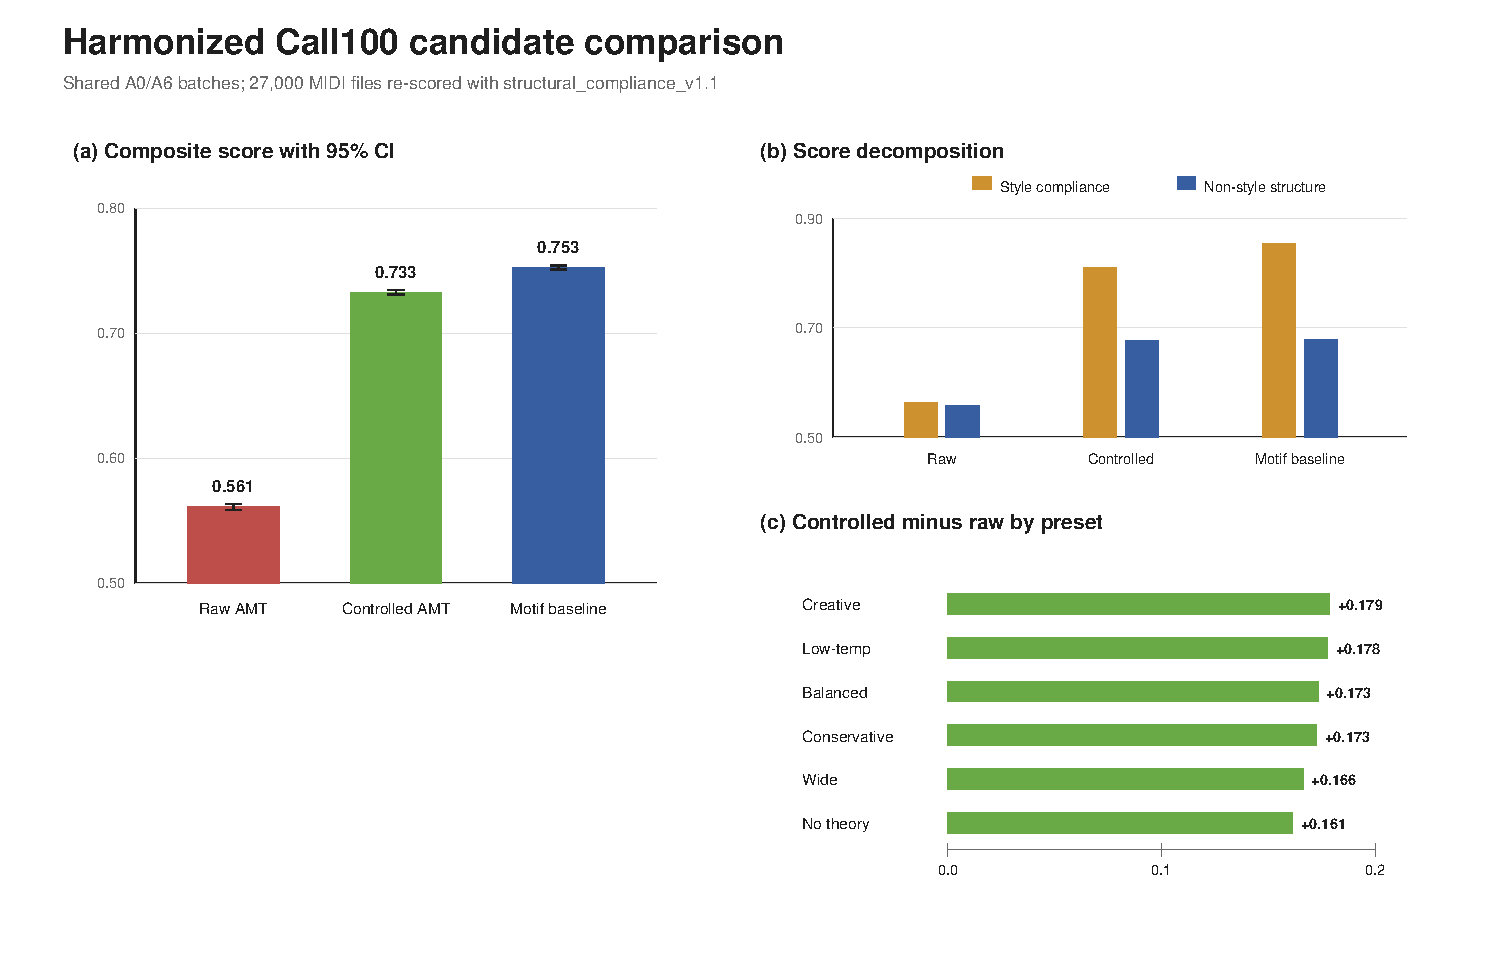
\includegraphics[width=0.96\linewidth]{figures/call100_candidate_level_comparison.pdf}
\caption{Harmonized Call100 comparison. Panel (a) reports SCC with 95\% confidence intervals, panel (b) separates style and non-style components, and panel (c) shows controlled-minus-raw SCC by preset.}
\label{fig:call100-candidate-level-comparison}
\end{figure}

Paired differences in Table~\ref{tab:bootstrap-tests} use the shared preset/call/trial key. Controlled minus raw is +0.171642 (95\% bootstrap CI [0.168923, 0.174287], $d_z=1.295$), while controlled minus motif is -0.020072. Numerical underflow is reported as $p<10^{-6}$, never $p=0$.

\begin{table}[htbp]
\centering
\caption{Paired candidate comparisons under the harmonized evaluator}
\label{tab:bootstrap-tests}
\small
\begin{tabular}{L{0.34\linewidth}r L{0.25\linewidth}r}
\toprule
Comparison & Mean difference & Bootstrap 95\% CI & paired $t$ $p$ \\
\midrule
\texttt{controlled - raw} & +0.171642 & [0.168923, 0.174287] & $<10^{-6}$ \\
\texttt{controlled - motif} & -0.020072 & [-0.022331, -0.017814] & $<10^{-6}$ \\
\texttt{motif - raw} & +0.191714 & [0.188850, 0.194556] & $<10^{-6}$ \\
\bottomrule
\end{tabular}
\end{table}

Controlled AMT exceeds raw AMT under every preset, but the motif baseline leads both score families. The claim is therefore improved structural compliance over raw AMT, not baseline dominance or listener preference.

\subsection{Controlled-AMT Module Ablation}
\label{subsec:controlled-amt-ablation}

The candidate-level Call100 experiment shows that controlled AMT improves over raw AMT, but not which components drive the gain. Table~\ref{tab:ablation-variants} defines a module-level ablation using the same 100 calls, six presets, seven variants, and 15 trials for each preset/variant/call combination:
\begin{equation}
100 \times 6 \times 7 \times 15 = 63000.
\end{equation}
The final validation confirms 63,000 actual rows, 4200 preset/variant/call groups, 15 trials per group, no missing SCC values, no missing response MIDI files, no unknown call IDs, and validation status \texttt{passed}.

\begin{table}[htbp]
\centering
\caption{Controlled-AMT ablation variants}
\label{tab:ablation-variants}
\small
\setlength{\tabcolsep}{4pt}
\begin{tabular}{lL{0.25\linewidth}L{0.50\linewidth}}
\toprule
Variant & Module added & Description \\
\midrule
A0 & Raw AMT & No external control. \\
A1 & Prompt cleaning & Only tail-repeat compression and prompt cleaning are enabled. \\
A2 & Repetition suppression & Adds generation-time repetition suppression and resampling. \\
A3 & Duration matching & Adds response duration and note-count matching. \\
A4 & Motif fallback & Adds motif fallback for empty or invalid neural output. \\
A5 & Style constraint & Adds pentatonic, two-bar, and 4/4 response style constraints. \\
A6 & Full controlled & All controlled-AMT modules are enabled. \\
\bottomrule
\end{tabular}
\end{table}

Table~\ref{tab:ablation-summary} reports SCC and its two predeclared components over 9000 samples per variant. A0 to A6 gains 0.171642 in SCC and 0.117733 in non-style structure.

\begin{table}[htbp]
\centering
\caption{Ablation summary by variant over Call100}
\label{tab:ablation-summary}
\small
\setlength{\tabcolsep}{4pt}
\begin{tabular}{lrrr}
\toprule
Variant & SCC & Style compliance & Non-style structure \\
\midrule
A0 raw AMT & 0.560968 & 0.563724 & 0.558971 \\
A1 prompt cleaning & 0.574265 & 0.566740 & 0.579714 \\
A2 repetition suppression & 0.610704 & 0.561879 & 0.646061 \\
A3 duration matching & 0.640526 & 0.575326 & 0.687740 \\
A4 fallback enabled & 0.640526 & 0.575326 & 0.687740 \\
A5 style constraint & 0.708929 & 0.764076 & 0.668994 \\
A6 full controlled & 0.732610 & 0.809814 & 0.676704 \\
\bottomrule
\end{tabular}
\end{table}

\begin{figure}[H]
\centering
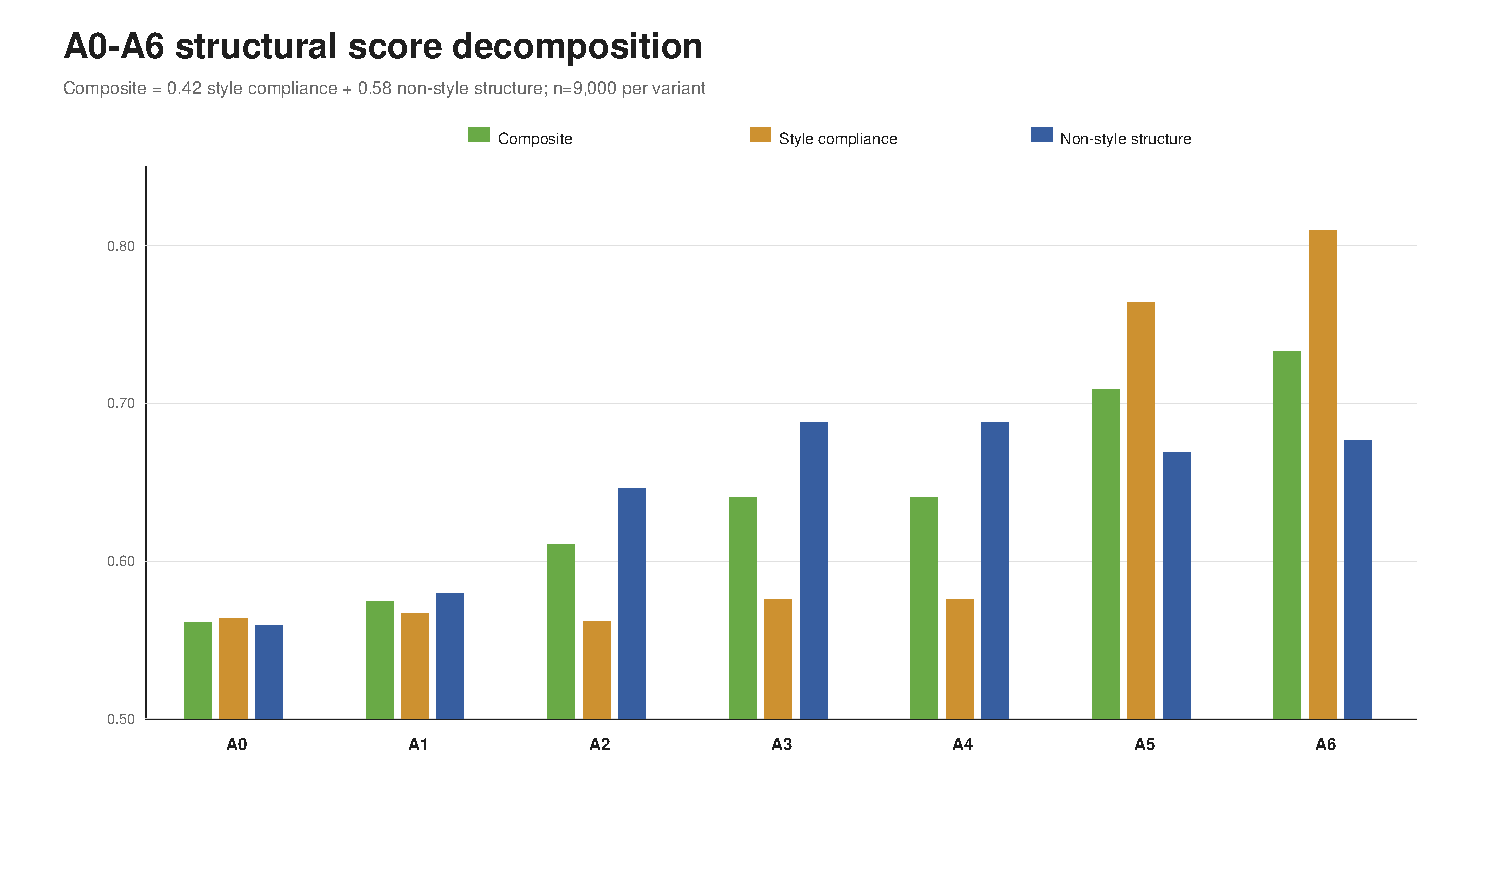
\includegraphics[width=0.92\linewidth]{figures/ablation_objective_scores.pdf}
\caption{A0--A6 score decomposition. Grouped bars report SCC, style compliance, and non-style structure over 9000 samples per variant.}
\label{fig:ablation-objective-scores}
\end{figure}

Figure~\ref{fig:ablation-objective-scores} makes the A5 mechanism visible: style compliance rises by 0.188750, while non-style structure decreases by 0.018746. The SCC increase at A5 is therefore a constraint-compliance manipulation check, not independent evidence of musical quality.

\begin{table}[htbp]
\centering
\caption{Stepwise module contributions to SCC}
\label{tab:ablation-contributions}
\small
\setlength{\tabcolsep}{4pt}
\begin{tabular}{llrcr}
\toprule
Step & Module added & Mean delta & 95\% CI & $p$ \\
\midrule
A1--A0 & Prompt cleaning & 0.013297 & [0.010832, 0.015736] & $<10^{-6}$ \\
A2--A1 & Repetition suppression & 0.036439 & [0.034068, 0.038919] & $<10^{-6}$ \\
A3--A2 & Duration matching & 0.029822 & [0.028143, 0.031398] & $<10^{-6}$ \\
A4--A3 & Motif fallback & 0.000000 & [0.000000, 0.000000] & n/a (all ties) \\
A5--A4 & Style constraint & 0.068403 & [0.066357, 0.070537] & $<10^{-6}$ \\
A6--A5 & Full controlled & 0.023681 & [0.022480, 0.024868] & $<10^{-6}$ \\
\bottomrule
\end{tabular}
\end{table}

\begin{figure}[H]
\centering
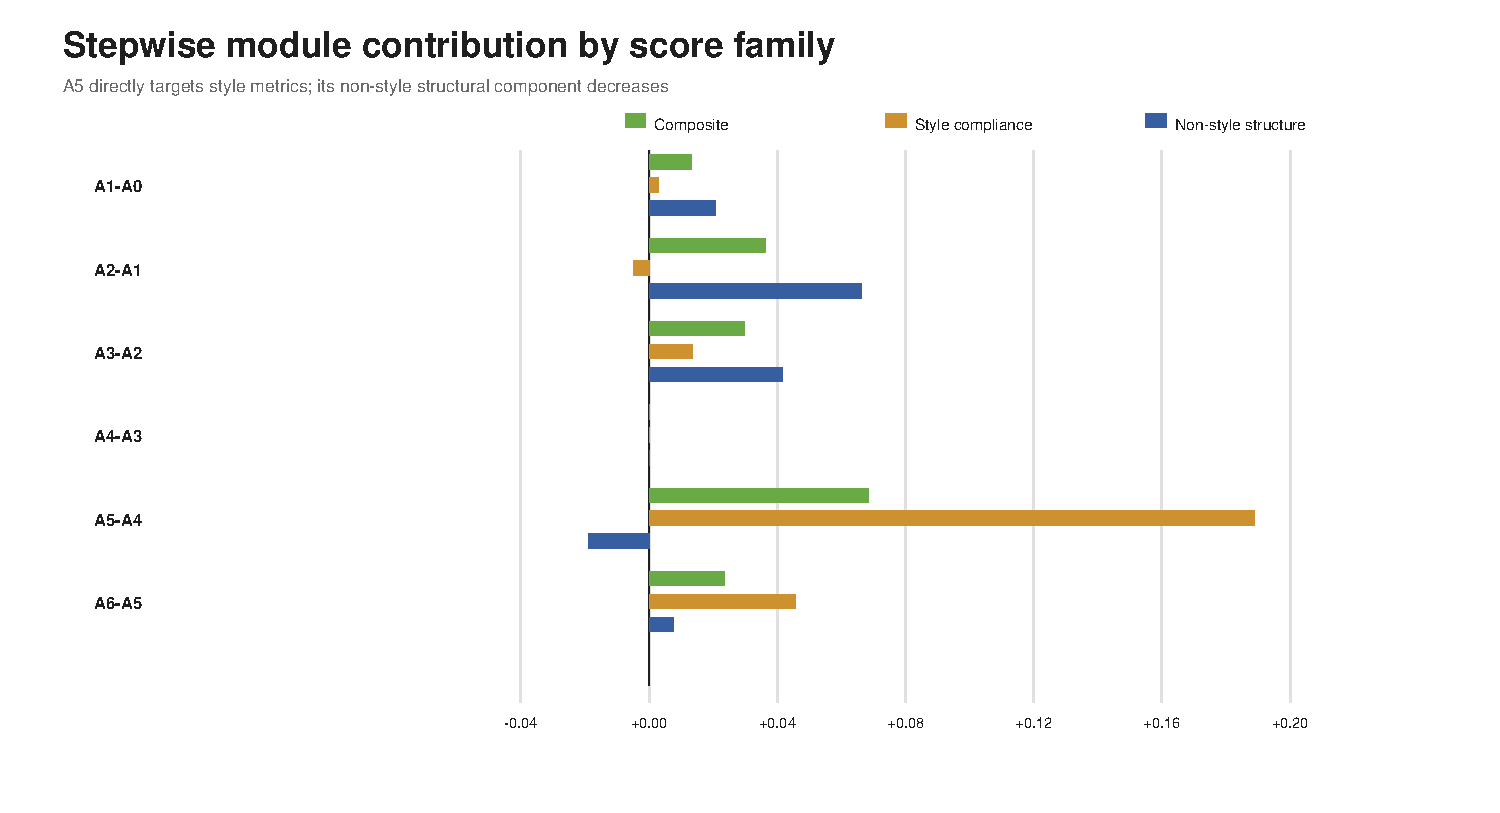
\includegraphics[width=0.92\linewidth]{figures/module_contribution_plot.pdf}
\caption{Stepwise changes in SCC, style compliance, and non-style structure. A5 directly optimizes the style family and slightly decreases the non-style family.}
\label{fig:module-contribution-plot}
\end{figure}

The fallback audit in Table~\ref{tab:fallback-audit} resolves the A3--A4 all-zero result. \texttt{event repair} counts individual rejected-token substitutions; \texttt{motif used} counts whole-phrase replacement.

\begin{table}[htbp]
\centering
\caption{Fallback activation audit over 9000 samples per variant}
\label{tab:fallback-audit}
\small
\begin{tabular}{lrrrr}
\toprule
Variant & Repair samples & Repair events & Empty before motif & Motif used \\
\midrule
A0 & 0 & 0 & 0 & 0 \\
A1 & 0 & 0 & 0 & 0 \\
A2 & 4236 & 6888 & 0 & 0 \\
A3 & 3712 & 5263 & 0 & 0 \\
A4 & 3712 & 5263 & 0 & 0 \\
A5 & 3712 & 5263 & 0 & 0 \\
A6 & 3712 & 5263 & 0 & 0 \\
\bottomrule
\end{tabular}
\end{table}

The evaluator assigns SCC=0 to an empty response. No A3 response was empty, so A4 had no eligible phrase and activated motif fallback zero times; if activated, the replacement MIDI would be evaluated after generation like every other output. All 9000 A3--A4 SCC differences are exactly zero and all 9000 response MIDI files are byte-identical. Within either variant, the 5288 samples without event repair average 0.643951, while the 3712 repaired samples average 0.635647. Therefore A4 is an unexercised safety branch in this run, not evidence that fallback is effective or ineffective.

\subsection{Direct MIDI-VAD Endpoint Benchmark}
\label{subsec:endpoint-benchmark}

The endpoint detector is evaluated directly by replaying all 100 Call100 files at 5 ms polling resolution. The final Note-Off of each isolated file is a reproducible proxy boundary. For each post-boundary deadline $d\in\{0.5,1.0,2.0\}$ s, at most one commit in $[T_{\mathrm{ref}}-0.1,T_{\mathrm{ref}}+d]$ is a true positive; other commits are false positives and an unmatched file is a false negative. The two-second deadline is the primary table, while all deadlines remain in the archive. This proxy does not replace human phrase-boundary annotation.

The main conditions compare adaptive MIDI-VAD with clustering/confirmation ablations and fixed 300, 500, and 800 ms silence thresholds. All fixed baselines retain the 80 ms cluster and 150 ms confirmation settings. Table~\ref{tab:endpoint-benchmark} reports 100 calls per condition; F1 intervals use 2000 call-level bootstrap resamples.

\begin{table}[htbp]
\centering
\caption{Call100 endpoint results at the two-second post-boundary deadline}
\label{tab:endpoint-benchmark}
\small
\setlength{\tabcolsep}{3.5pt}
\begin{tabular}{lrrrrrr}
\toprule
Condition & Precision & Recall & F1 & Premature & Cancel rate & Median error s \\
\midrule
Adaptive full & 0.624 & 0.830 & 0.712 & 38 & 0.070 & 0.796 \\
No clustering & 0.610 & 0.830 & 0.703 & 42 & 0.087 & 0.796 \\
No confirmation & 0.597 & 0.860 & 0.705 & 49 & 0.000 & 0.632 \\
Neither & 0.571 & 0.840 & 0.680 & 53 & 0.000 & 0.632 \\
Fixed 300 ms & 0.250 & 0.760 & 0.376 & 228 & 0.374 & 0.330 \\
Fixed 500 ms & 0.427 & 0.880 & 0.575 & 118 & 0.116 & 0.500 \\
Fixed 800 ms & 0.575 & 0.920 & 0.708 & 68 & 0.130 & 0.793 \\
\bottomrule
\end{tabular}
\end{table}

\begin{figure}[H]
\centering
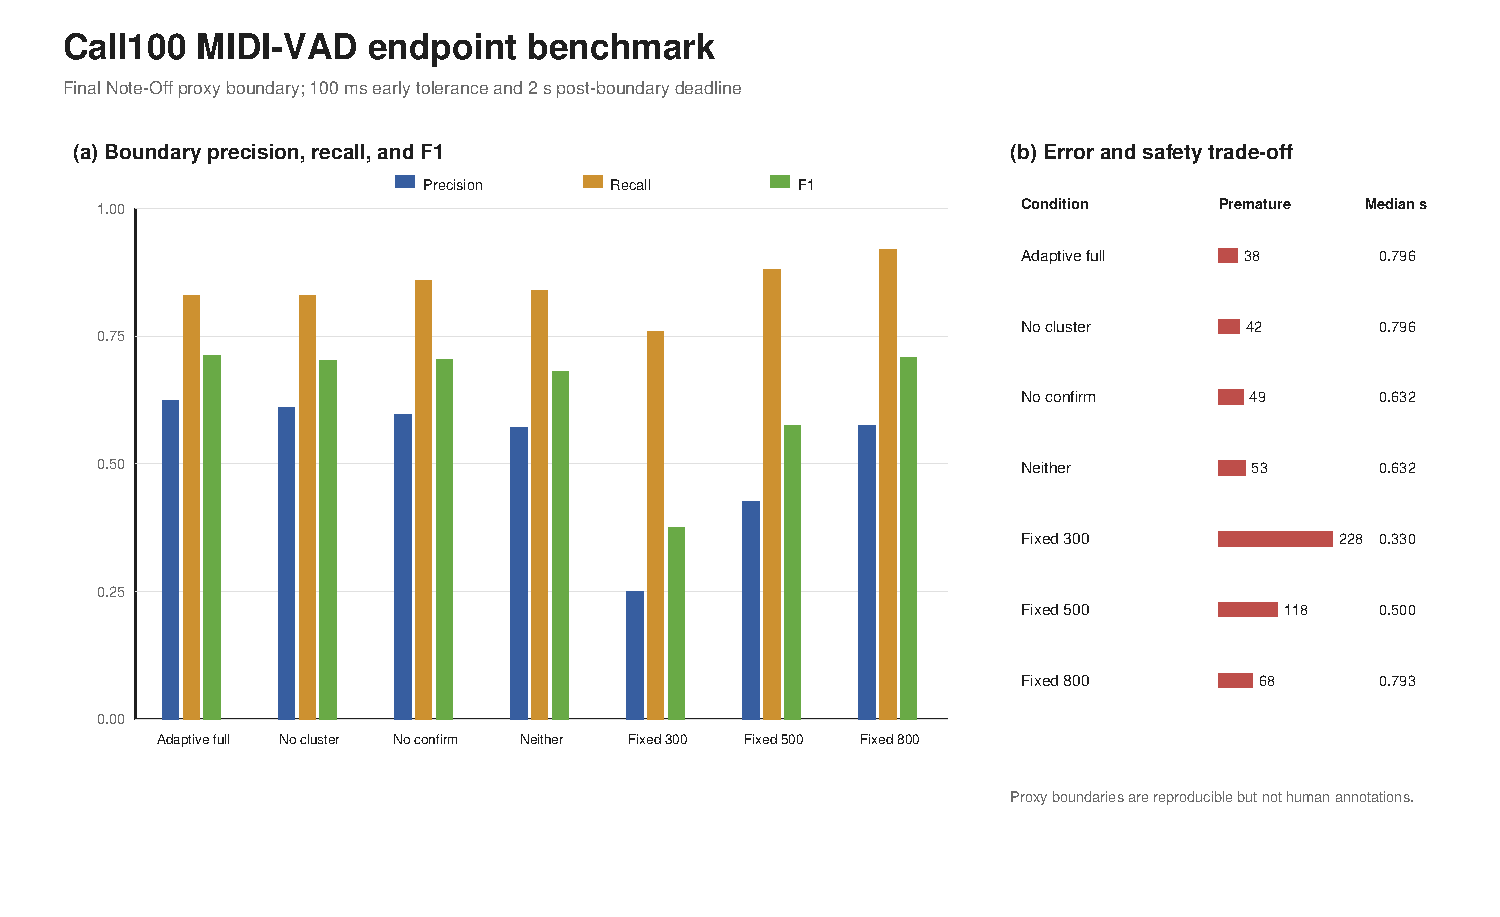
\includegraphics[width=0.96\linewidth]{figures/endpoint_benchmark.pdf}
\caption{Direct endpoint benchmark. Panel (a) reports precision, recall, and F1; panel (b) shows premature commits and median signed boundary error.}
\label{fig:endpoint-benchmark}
\end{figure}

Adaptive full yields F1=0.712 (95\% CI [0.638, 0.784]), comparable to fixed 800 ms at 0.708 [0.646, 0.767], while reducing premature commits from 68 to 38; the overlapping intervals do not establish superiority. Its recall is 0.14, 0.58, and 0.83 at the 0.5, 1.0, and 2.0 s deadlines, respectively, exposing the latency cost of conservative segmentation. Cluster-window sensitivity gives F1 values 0.703, 0.715, 0.712, and 0.704 at 0, 40, 80, and 120 ms. Confirmation sensitivity gives 0.705, 0.695, 0.712, and 0.728 at 0, 75, 150, and 250 ms, while median error rises from 0.632 to 0.705, 0.796, and 0.896 s. Thus 80/150 ms is a middle operating point, not a uniquely optimal constant.

\subsection{Runtime Latency Logging and Scheduler Replay}
\label{subsec:latency-logging}

SCC does not characterize scheduler responsiveness. The latency experiment therefore replays actual local AMT decoding timings collected during the A6 runs. The machine is a Lenovo 82JQ running 64-bit Windows 11 Pro, with an AMD Ryzen 7 5800H (8 cores/16 logical processors), 15.86 GiB physical RAM, and an NVIDIA GeForce RTX 3060 Laptop GPU with 6144 MiB VRAM. L0 starts decoding at endpoint commit. L1 overlaps decoding only with the confirmation interval, so $\Delta T_{\mathrm{preload}}=\Delta T_{\mathrm{confirm}}=150$ ms; no additional 250 ms horizon exists. Both use an 80 ms micro-buffer and underrun deadline. Inference timings are observed, whereas endpoint-to-first-MIDI values are deterministic scheduler replay rather than direct live-performance measurements.

The primary latency metric is endpoint-to-first-MIDI latency:
\begin{equation}
L_{\mathrm{first}} = t_{\mathrm{first\_midi\_out}} - t_{\mathrm{endpoint\_commit}}.
\end{equation}
This metric measures the delay between the confirmed phrase endpoint and the first scheduled MIDI response event.

\begin{table}[htbp]
\centering
\caption{Runtime latency comparison between preload-off and preload-on conditions}
\label{tab:latency-condition}
\small
\setlength{\tabcolsep}{4pt}
\begin{tabular}{lrrrrrr}
\toprule
Condition & Samples & Mean ms & P50 ms & P95 ms & P99 ms & Underrun \\
\midrule
L0 preload off & 9000 & 161.303 & 136.455 & 323.521 & 479.574 & 20.744\% \\
L1 preload on & 9000 & 91.721 & 80.000 & 173.521 & 329.574 & 5.244\% \\
\bottomrule
\end{tabular}
\end{table}

\begin{table}[htbp]
\centering
\caption{Paired latency reduction from speculative preload}
\label{tab:preload-paired-reduction}
\small
\setlength{\tabcolsep}{5pt}
\begin{tabular}{lrrc}
\toprule
Comparison & Paired samples & Mean reduction ms & 95\% CI \\
\midrule
L1 preload on vs. L0 preload off & 9000 & 69.582 & [68.865, 70.263] \\
\bottomrule
\end{tabular}
\end{table}

\begin{figure}[H]
\centering
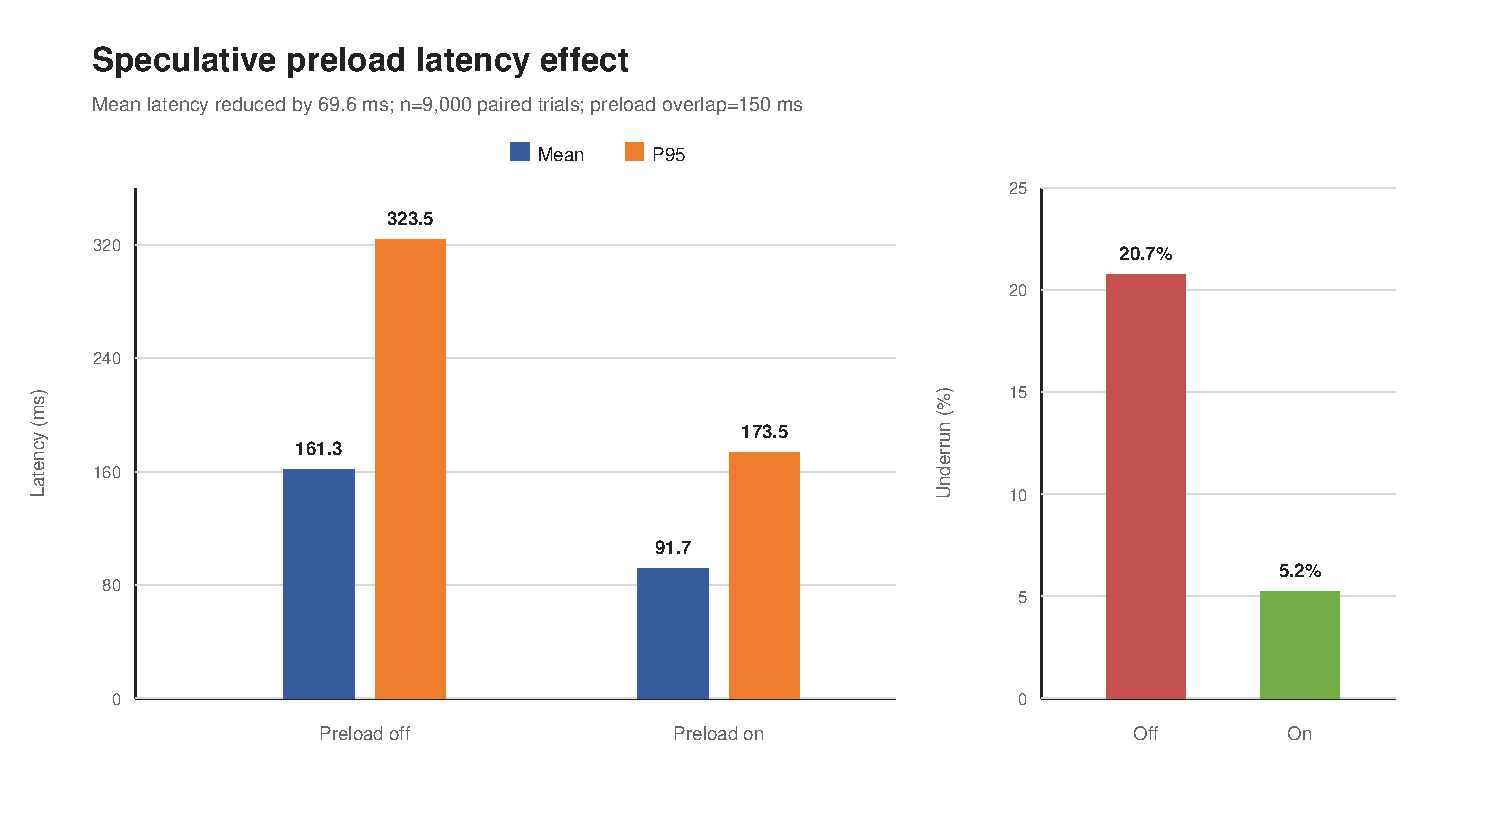
\includegraphics[width=0.92\linewidth]{figures/preload_latency_chart.pdf}
\caption{Scheduler-replay comparison with preload off and with 150 ms of pre-commit overlap. The left panel reports mean and P95 endpoint-to-first-MIDI latency; the right panel reports buffer-underrun rate.}
\label{fig:preload-latency-chart}
\end{figure}

Tables~\ref{tab:latency-condition} and~\ref{tab:preload-paired-reduction}, together with Figure~\ref{fig:preload-latency-chart}, show the replay results. All 9000 paired differences favor preload; an exact two-sided paired sign test gives $p<10^{-6}$. Preload reduces mean endpoint-to-first-MIDI latency from 161.303 ms to 91.721 ms, reduces P95 from 323.521 ms to 173.521 ms, and lowers buffer-underrun rate from 20.744\% to 5.244\%. This improves scheduled post-endpoint responsiveness by moving up to 150 ms of decoding into the candidate-confirmation interval; it does not reduce intrinsic AMT decoding time.

\subsection{Dataset Source Robustness and Failure-Case Analysis}
\label{subsec:robustness-failure}

Table~\ref{tab:source-origin-summary} applies the harmonized evaluator to source groups. The original Call50 subset remains easier than the added POP909 subset.

\begin{table}[htbp]
\centering
\caption{Performance by source dataset and origin}
\label{tab:source-origin-summary}
\begin{tabular}{llrr}
\toprule
Grouping field & Value & Samples & Mean SCC \\
\midrule
source dataset & \texttt{calls\_50} & 13500 & 0.702215 \\
source dataset & \texttt{POP909} & 13500 & 0.661958 \\
\midrule
origin & \texttt{artificial\_stress} & 2700 & 0.725250 \\
origin & \texttt{real\_public\_dataset} & 10800 & 0.696456 \\
origin & \texttt{public\_midi\_extract} & 13500 & 0.661958 \\
\bottomrule
\end{tabular}
\end{table}

This difference does not indicate failure on POP909; it shows that the added public excerpts are harder. The POP909 subset has a higher average maximum interval, 12.093 versus 8.360 for \texttt{calls\_50}, and a higher average note count, 15.905 versus 13.588, increasing the difficulty of response planning and duration matching.

Category extremes in Table~\ref{tab:category-summary} similarly identify sparse and rubato inputs as difficult under SCC.

\begin{table}[htbp]
\centering
\caption{Examples of high- and low-scoring categories}
\label{tab:category-summary}
\small
\begin{tabular}{L{0.35\linewidth}rrL{0.31\linewidth}}
\toprule
Category & Samples & Mean SCC & Interpretation \\
\midrule
\texttt{pentatonic\_clear\_motif} & 270 & 0.775829 & Clear motif and stable scale structure. \\
\texttt{modal\_question} & 270 & 0.774319 & Clear question-like phrasing and cadential target. \\
\texttt{syncopation} & 270 & 0.753149 & Distinct rhythmic profile remains structurally manageable. \\
\midrule
\texttt{expressive\_rubato} & 2160 & 0.632543 & Free timing increases rhythm and duration-matching difficulty. \\
\texttt{sparse\_short} & 1350 & 0.620874 & Low input information makes structural filling less stable. \\
\texttt{sparse\_cadential} & 270 & 0.618459 & Sparse cadential fragments often lead to short or weak responses. \\
\bottomrule
\end{tabular}
\end{table}

For A6, event repair occurs in 3712/9000 samples (41.24\%; 5263 repaired events), but whole-phrase motif fallback occurs zero times. Reporting the former as a ``fallback rate'' caused the earlier 41.46\% ambiguity; the public schema now stores \texttt{event\_repair\_count} and \texttt{motif\_fallback\_used} separately.

\subsection{Anonymous Blind Listening Study}
\label{subsec:blind-listening-study}

\paragraph{Stimuli and procedure.}
The subjective experiment used a single-stimulus, fully randomized design. Each participant rated eight anonymous piano-rendered clips constructed from four call contexts: two POP909 excerpts and two artificial stress cases. Within each context, both conditions used the same call and only the response differed. Two contexts compared raw AMT (A0) with controlled AMT (A4), while two compared the motif-transformation baseline with full controlled AMT (A6). A4 cumulatively activates prompt cleaning, repetition suppression, duration matching, and a fallback-capable branch; A6 additionally activates the style and full-theory controls. All responses used the \texttt{pentatonic\_conservative} preset. For each call--condition combination, the displayed response was the trial whose SCC was closest to the median of 15 trials. Every selected response had \texttt{event\_repair\_count}=0 and \texttt{motif\_fallback\_used}=0, so no listening stimulus contained event repair or whole-phrase replacement.

Each participant evaluated all eight clips in an independently randomized order. The interface disclosed neither model identity nor condition label and showed no MIDI visualization. For each item, listeners could play synchronized renderings of the full call plus response, the call alone, and the response alone. They then answered four mandatory questions about (1) transition fluency, (2) phrase development and closure, (3) rhythmic and musical correspondence with the call, and (4) overall acceptability. Each question used a forced-choice four-point scale from 1 to 4, with no neutral option. Playback counts, presentation position, per-item dwell time, and total study duration were recorded.

\paragraph{Participants and quality control.}
Recruitment was anonymous and conducted through WeChat using the mainland-China deployment. Participants acknowledged that their anonymous ratings would be used for academic analysis before starting, and no direct personal identifiers were requested. The frozen export contained 44 complete submissions and 1,408 rating rows, exactly 32 rows per submission. Before unblinding, two submissions were excluded because at least one item had no recorded playback, and the later of two submissions sharing one session identifier was removed. This left 41 participants and 1,312 ratings for the primary analysis. One participant used the same score throughout; this response was retained under the locked rule, and excluding it in sensitivity analysis did not change either conclusion. Among included participants, 15 reported 0--2 years, 17 reported 3--5 years, and 9 reported more than 5 years of musical experience; 25 reported high and 16 low familiarity with improvisation. Listening devices were headphones ($n=23$), phones ($n=13$), and speakers ($n=5$). Median completion time was 322 seconds.

\paragraph{Analysis.}
For each participant and comparison family, ratings were averaged over the four questions and two matched call contexts. Primary effects are paired participant-level mean differences, defined as controlled minus comparator. Confidence intervals were obtained with 50,000 participant-bootstrap draws, and two-sided $p$ values with 200,000 sign-flip permutations. Cohen's $d_z$ summarizes paired effect size. A secondary linear model adjusted for presentation index and call-pair fixed effects while including participant fixed effects and participant-clustered standard errors. The four questions showed high internal consistency across participant-item observations (Cronbach's $\alpha=0.939$).

\begin{table}[htbp]
\centering
\caption{Blind-listening results on a four-point scale ($N=41$). Differences are controlled minus comparator; confidence intervals use participant bootstrap resampling.}
\label{tab:blind-listening-results}
\scriptsize
\begin{tabular}{L{0.25\linewidth}rrL{0.25\linewidth}r}
\toprule
Comparison & Comparator & Controlled & Difference (95\% CI) & $p_{\mathrm{perm}}$ \\
\midrule
Controlled A4 $-$ raw AMT & 2.945 & 2.787 & $-0.159$ [$-0.326$, 0.006] & 0.0785 \\
Controlled A6 $-$ motif baseline & 2.256 & 1.909 & $-0.348$ [$-0.534$, $-0.162$] & 0.0009 \\
\bottomrule
\end{tabular}
\end{table}

\paragraph{Results.}
Table~\ref{tab:blind-listening-results} does not support a perceptual advantage for controlled AMT on the selected stimuli. In the A4 comparison, controlled AMT was rated 0.159 points below raw AMT, but the interval included zero ($d_z=-0.289$, $p=0.0785$). After adjustment for presentation position and matched call pair, the estimated difference remained similar at $-0.164$ (95\% CI [$-0.352$, 0.025], approximate $p=0.090$). The correct interpretation is uncertainty rather than equivalence or superiority.

In the A6 comparison, controlled AMT was rated 0.348 points below the motif baseline (95\% CI [$-0.534$, $-0.162$], $d_z=-0.570$, $p=0.0009$). The adjusted estimate was $-0.349$ (95\% CI [$-0.567$, $-0.131$], approximate $p=0.0017$), preserving the conclusion after accounting for order and call pair. Ratings increased by approximately 0.038 points per later presentation position (95\% CI [0.009, 0.068]), which justifies retaining order in the adjusted model but does not explain the condition contrast. Excluding the one straight-line participant yielded nearly identical differences ($-0.163$ and $-0.356$).

Across the eight fixed stimuli, SCC and mean human rating showed little descriptive alignment (Pearson $r=-0.054$; Spearman $\rho=0.071$). With only eight selected stimuli this is exploratory. Structural compliance improves over raw AMT at scale, but these exemplars do not show corresponding listener preference; the motif baseline is preferred to A6 on this restricted test.

\subsection{Interpretation and Scope of Evaluation}
\label{subsec:subjective-evaluation-scope}

The endpoint benchmark uses file-end proxies rather than human boundaries, motif fallback never activates in A0--A6, and scheduler replay does not measure faster AMT inference. The blind study contains 41 analyzed participants from one Chinese social channel, four contexts, one preset, and eight fixed, repair-free stimuli. No live co-performance user study is included, so perceived turn taking and broader musical usefulness remain unverified.

\section{Conclusion}
\label{sec:conclusion-future-work}

The primary contribution is an external method that places adaptive turn detection, phrase control, and speculative scheduling around a frozen offline AMT. Direct endpoint replay shows a precision--latency trade-off rather than universal segmentation accuracy. Shared-batch evaluation raises SCC from 0.560968 to 0.732610 and non-style structure from 0.558971 to 0.676704; A5's larger style gain is explicitly separated from that evidence. A 150 ms overlap lowers replayed scheduler latency from 161.303 to 91.721 ms, but the listening study does not establish perceptual superiority. Future work should use human-labeled phrase boundaries, live interaction, and broader pre-registered listening samples.

\section*{Data and Code Availability}
\label{sec:data-code-availability}

The research code, paper source, trial-level structural metrics, endpoint and latency summaries, aggregate listening results, and release documentation are available in the \href{https://github.com/MickeyWzt/real-time-midi-call-response}{public GitHub repository}. The reproducibility archive corresponding to this manuscript is \href{https://github.com/MickeyWzt/real-time-midi-call-response/releases/tag/v1.1.0}{GitHub release v1.1.0}. Zenodo archives the release under the stable \href{https://doi.org/10.5281/zenodo.20838083}{all-versions concept DOI}; the release page links its exact version DOI. A browsable \href{https://mickeywzt.github.io/real-time-midi-call-response/}{project page} is also available.

The public archive includes the implementation, exact score specification, path-redacted trial metrics, source hashes, statistical summaries, and tests needed to inspect the reported structural, endpoint, scheduling, and aggregate listening results. Participant-level response exports, exclusion identifiers, private answer keys, and deployment credentials are retained privately. Large or license-sensitive runtime artifacts, including pretrained model weights, third-party audio tools, sample libraries, source datasets, and generated per-run MIDI batches, are not redistributed and should be obtained separately under their respective licenses.


\section*{AI Tool Usage Statement}
\label{sec:ai-tool-usage}

AI tools were used in this project as auxiliary research, writing, and programming support. This disclosure refers to general-purpose AI assistance used during project preparation; the autoregressive Transformer system evaluated in this paper is part of the research object itself and is described separately in the methodology and experiments.

The authors used OpenAI ChatGPT/Codex in three main places. First, during software development, AI assistance was used to inspect Python and MIDI-processing code, identify possible implementation errors, debug LaTeX or Python issues, and draft small validation or analysis procedures. All code execution, experiment running, and result validation were performed and checked by the authors. Second, during manuscript preparation, AI assistance was used to improve English wording, reorganize paragraphs, refine LaTeX formatting, and make tables and figure descriptions clearer. Third, during result reporting, AI assistance was used to help summarize verified CSV and log outputs and convert checked numerical results into concise academic prose.

AI tools were not used to fabricate experimental data, replace the Call100 or blind-listening evaluations, make unsupervised final research decisions, or generate references accepted without checking. All numerical claims, tables, figures, citations, and final conclusions were reviewed by the authors against the frozen experiment outputs, source code, and cited literature.


\bibliographystyle{plainnat}
\bibliography{references}

\end{document}
